Tas, ko sauc par ķēdi plašākā sabiedrībā, tik stipri atšķirās no Bitcoin tehniskā apraksta\cite{nakamoto08} dotās definīcijas, ka tā vairs nav izmantojama. 
Lielākoties par ķēdi tiek saukta decentralizēta norēķinu sistēma, tomēr pa virsu šīm norēķinu sistēmām tiek veidoti arī citi servisi, kuriem ar naudas pārskaitījumiem nav nekāda sakara, piemēram, domēna vārdu reģistra, sertifikātu autoritātes, vēlēšanu un citi servisi.\cite{namecoin}
Turklāt esošām ķēžu implementācijām ir tik daudzveidīga funkcionalitāte, ka ir grūti spriest, kādās ir vispārīgas ķēdes īpašības.
Šajā nodaļā aplūkosim ar ķēdēm saistītas tēmas \textemdash{} decentralizētas sistēmas, digitālas valūtas un blokķēdē izmantotās datu struktūras. Beigās tiek aplūkotas konkrētas ķēdes realizācijas.

\subsection{Digitāla valūta}
Naudas atkārtota iztērēšana (double spending) ir kritiskākā digitālu valūtu problēma, kas ir analoģiska fiziskas naudas viltošanai, bet, tā kā digitāla valūta pēc savas būtības glabājas uz datora, tad to ir viegli nokopēt neskaitāmos eksemplāros. Vienīgais veids kā novērst problēmu ir, ja pārdevējs nelaiž pircēju ārā no veikala, kamēr nav saņēmis apstiprinājumu par naudas īpašnieka maiņu no vienota patiesības avota.\cite{frankel96}

Mūsdienās par patiesības avotu parasti kalpo kāda centrāla organizācija, piemēram, Visa vai PayPal, tomēr vienots patiesības avots var būt arī jebkurš izkliedētas sistēmas dalībnieks, ja visi tās dalībnieki laika gaitā pieņems vienādu stāvokli.
Ar parakstītu ziņojumu palīdzību ir iespējams izveidot autorizētus maksājuma pieprasījumus, un šeit nav būtiskas atšķirības starp centralizētu un decentralizētu risinājumu. Savukārt sistēmai saņemot divus pieprasījumus, no kuriem katrs atsevišķi ir derīgs, bet abi kopā izpildīties nevar, ir jāpieņem lēmums: kurš izpildās un kurš ne.

Centralizētās sistēmās hronoloģiski pirmais pieprasījums tiktu izpildīts, bet vēlākais tiktu atteikts. Diemžēl decentralizētā gadījumā nav objektīva secība, kurā pienāk ziņojumi. Ir nepieciešams vienprātības (consensus) algoritms, kas garantēs, ka visi maksājuma pieprasījumi tiek sakārtoti vienādā secībā visiem dalībniekiem, nodrošinot arī vienādu virsgrāmatas stāvokli.
Turklāt algoritmam jābūt noturīgam pret cenzūru un sabotāžu, lai tas būtu lietojams decentralizētā vidē.

\subsection{Datu struktūras}
Šajā nodaļā aplūkosim datu struktūras, kas ļauj pārliecināties par datu integritāti. Pieņemsim, ka ir nepieciešams iegūt lielu datu apjomu un ir uzticams avots, no kura iegūt hash vērtību, pret kuru var pārbaudīt, ka dati nav mainīti. 
%kas ir hash?

Naivais veids būtu aprēķināt hash no visiem datiem un salīdzināt pret uzticamā avota sniegto hash vērtību. Problēma šādā pieejā ir tāda, ka, iegūstot nedaudz atšķirīgus datus, tie visi ir jāizmet un jāmeklē cits datu ieguves avots. Aplūkosim metodi, kas optimizē nepieciešamo komunikācijas daudzumu un dod iespēju iegūt datus no dažādiem avotiem vienlaicīgi.

Sadalīsim datus vairākās daļās un katrai daļai aprēķināsim hash vērtību. Tad tiek aprēķināts hash no visām iepriekš iegūtajām hash vērtībām, un šo izmanto par galveno (saknes) hash vērtību, kas iegūta no uzticamā avota. Skatīt attēlu~\ref{fig:hash-list}.

\begin{figure}[htpb]
    \centering
    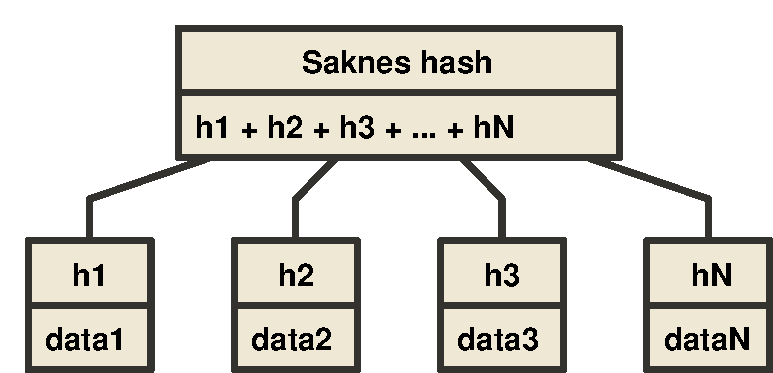
\includegraphics[scale=0.5]{teorija/hash-list.pdf}
    \caption{Hash saraksts}
    Dati tiek sadalīti vairākās daļās, katrai daļai tiek aprēķināta hash vērtība. Saknes hash tiek aprēķināts no atsevišķo daļu hash vērtībām.
\label{fig:hash-list}
\end{figure}

Tagad pirms sākt datu ieguvi tiek iegūts saraksts ar hash vērtībām sadalītajiem datiem. Ievēro, ka informācijas apjoms, kas jāpārsūta šajā gadījumā ir ievērojami mazāks par visu datu apjomu. Sarēķina, vai hash no saraksta atbilst tam, kas tiek iegūts no drošā avota, ja rodas nesakritība, tad ir skaidrs, ka nav vērts sākt pašu datu lejuplādi. Kad ir veiksmīgi iegūts pareizais hash saraksts, tad lejupielādi datiem var veikt no vairākiem avotiem, katram avotam prasot savus datu gabaliņus, kā arī uzreiz izķerot kļūdas.

Līdzīgi mehānismi tiek izmantoti decentralizētos failu apmaiņas protokolos piemēram, BitTorrent. Metode strādā ļoti labi, ja dati laika gaitā ir nemainīgi, tomēr mainīgiem datiem būtu neparocīgi katru reizi pārrēķināt galveno hash vērtību, jo tad tā ir jāmaina uzticamajam avotam. Aplūkosim metodi, kas ļauj ar nemainīgu galveno hash vērtību validēt datus, kuri regulāri tiek pagarināti, bet vēsture paliek nemainīga.

Aplūkojamā datu struktūra sastāv no blokiem, kuri sastāv no datiem un iepriekšējā bloka hash vērtības.\cite{nakamoto08} Pats pirmais bloks, kas satur sākotnējo vērtību, nesatur sevī hash vērtību, un šo bloku sauc arī par \textit{genesis block}. 
%genesis block - izcelsmes / sākotnējais bloks
Datu struktūra ir līdzīga saistītajam sarakstam, bet atšķirība ir tāda, ka nav iespējams mainīt bloka saturu vai ievietot pa vidu vēl kādu bloku. Skatīt attēlu~\ref{fig:hash-chain}.


\begin{figure}[htpb]
    \centering
    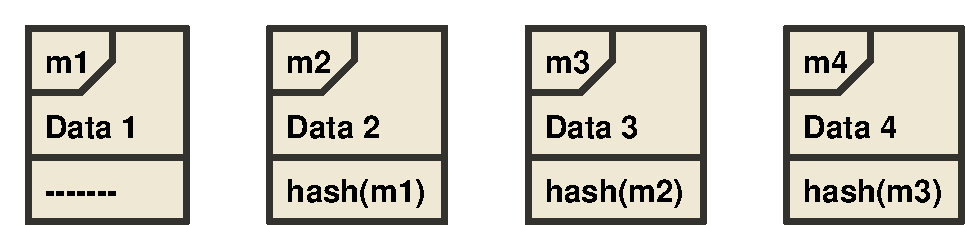
\includegraphics[scale=0.5]{teorija/hash-chain.pdf}
    \caption{Hash ķēde}
    Katrs hash ķēdes ziņojums $m_i$ sastāv no sev raksturīgajiem datiem $d_i$ un
    iepriekšējā posma $m_{i-1}$ hash vērtības.
\label{fig:hash-chain}
\end{figure}

Piemēram, pamainot otrā bloka datu vērtību, mainās bloka hash, un tas vairs nesakrīt ar trešajā blokā ierakstīto hash vērtību. Savukārt, izmainot trešajā blokā ierakstīto otrā bloka hash vērtību, izmainās trešā bloka hash, salaužot ceturto bloku. Tātad, lai izmainītu datus blokā $i$ ir jāizmaina visi bloki, kuri seko $i$. Tieši šī datu struktūra tiek izmantota visās blokķēžu implementācijās.

\subsection{Izkliedētā skaitļošana (distributed computing)}
Izkliedētās skaitļošanas pirmssākumi meklējami failu apmaiņā starp vienaudžiem. Mūsdienās populārākais protokols šī mērķa sasniegšanai ir BitTorrent. Ja kāds fails tīklā kļūst populārs, tad ir pamats ticēt, ka tas nevar no turienes pazust, jo veiksmīgākie mēģinājumi cīnīties pret dalīšanos BitTorrent tīklā ir saistīti ar uzbrukumiem tādiem serveriem, kas uztur sarakstu ar tīklā atrodamajiem failiem. Tomēr ir ieviesti strādājoši paplašinājumi BitTorrent protokolam, kas pilda minēto serveru funkciju decentralizētā vidē.\cite{pouwelse08} Tā kā sistēma ir publiski pieejama un noturīga pret cenzūru, tad tā ir piemērota bāze decentralizētas finanšu infrastruktūras radīšanai. Atliek atrisināt problēmu, kur maksājuma pieprasījumiem jābūt vienā secībā, turklāt šī secība nedrīkst mainīties. Tehniskā līmenī ķēde risina tieši šo problēmu.

Piebildīsim, ka ļaundariem paveras jauns uzbrukuma virziens, kas nebija aktuāls BitTorrent gadījumā, jo sistēmā, kuru veidojam, nedrīkst pieļaut, ka virsotnes ignorē legālas transakcijas, bet, no otras puses, ļaundaris var uzģenerēt lielu skaitu legālu transakciju, efektīvi veicot DoS uzbrukumu. Vairums ķēžu risina šo problēmu iekasējot nelielu komisiju par katru transakciju.

Aprakstīsim Bizantijas vienošanās problēmu (Byzantine agreement, Byzantine generals problem).
Pieņemsim, ka ir sistēma kas sastāv no tīklā saslēgtiem datoriem, kuri sazinās savā starpā sūtot ziņojumus. Mērķis ir vienoties par koordinētu tālāko rīcību, kas ir atkarīga no ārējiem apstākļiem, kuri iepriekš nav zināmi. Uzdevumu padara grūtu tas, ka starp datoriem var būt arī tādi, kas ļaunprātīgi cenšas sabotēt vienotu rīcību.
Problēmas atrisinājums ir vienprātības algoritms, kuram izpildās divas īpašības.
\begin{enumerate}
    \item Datoram izpildot algoritmu tiek pieņemts tāds pats lēmums, kā citiem datoriem, kuri izpilda algoritmu.
    \item Neliels daudzums ar ļaunprātīgiem datoriem nespēj ietekmēt pieņemto lēmumu.
\end{enumerate}\cite{lamport82}
Turpmāk datoru šīs problēmas kontekstā sauksim par \textbf{virsotni} (node), jo šis termins tiek lietots ar ķēdēm saistītā literatūrā. Veiksim arī citas nelielas modifikācijas dotajam uzdevumam.
Pēc katra pieņemtā lēmuma tīkla stāvoklis būs mainījies, un lēmuma pieņemšanu būs nepieciešams atkārtot. Teiksim, ka katram pieņemtajam lēmumam $x$ ir indekss $i$. Virsotne var droši \textbf{publicēt} vērtību $x$ pozīcijā $i$, ja visiem iepriekšējiem indeksiem ir publicēts kāds lēmums un virsotne ir pārliecināta, ka arī citas virsotnes laika gaitā publicēs vērtību $x$ pozīcijā $i$.\cite{mazieres15} Tādējādi mēs neprasām, lai visas virsotnes pieņemtu vienotu lēmumu vienlaicīgi, bet gan to, lai vienots lēmums eksistētu. Šāda modifikācija noteikti ir nepieciešama, jo decentralizētā vidē nav pat zināms dalībnieku skaits un viens ļaundaris var netraucēti izlikties par vairākām virsotnēm.
Tādēļ arī otro nosacījumu padarīsim spēcīgāku un skaidrāku, prasot, lai jebkāds daudzums ar ļaunprātīgām virsotnēm nespēj ietekmēt pieņemto lēmumu.
Turklāt kļūst skaidrs, ka mūsu gadījumā demokrātiska lēmuma pieņemšana nav risinājums, tāpēc aplūkosim populārākos līdz šim piedāvātos vienprātības algoritmus.

\subsubsection{Pierādījums ar darbu (Proof of work)}
Virsotnes darbojas pēc sekojoša principa:\cite{nakamoto08}
\begin{enumerate}
    \item Jaunās transakcijas tiek paziņotas visām virsotnēm.
    \item Katra virsotne izvēlas transakcijas, kuras iekļaut jaunajā blokā.
    \item Katra virsotne risina skaitliski sarežģītu problēmu, kas padarītu izvēlēto bloku legālu.
    \item Kad kāda virsotne atrisina problēmu, tad tā paziņo atrasto bloku visām pārējām virsotnēm.
    \item Pārējās virsotnes pārbauda, vai atrastais bloks ir legāls.
    \item Pārējās virsotnes turpina risināt sarežģīto problēmu pa virsu jaunajam blokam.
\end{enumerate}
Trešais punkts nodrošina to, ka ļaundarim nav vērts izlikties par vairākām virsotnēm, jo spēja radīt jaunus blokus ir proporcionāla skaitļošanas jaudai, bet ļaundara skaitļošanas jauda ir ierobežota.

Sesto punktu nepieciešams paskaidrot sīkāk. Par ķēdes \textbf{svaru} sauksim vidējo skaitļošanas darbu, kāds nepieciešams, lai atrastu visus blokus šajā ķēdē. Pareizā vēsture ir tā, kurai ir vislielākais svars. Par bloka atrašanu virsotnes īpašniekam palielinās bilance, tāpēc visas virsotnes ir motivētas taisīt jaunus blokus uz pareizās vēstures. Kad uz pareizās vēstures tiek atrasts bloks, tās svars palielinās, un šī vēsture kļūst vēl pareizāka. Ja divām vēsturēm ir līdzīgs svars, tad daļa no virsotnēm meklēs nākamo bloku uz vienas vēstures, bet daļa uz otras. Tai vēsturei, kurai pirmajai atradīs nākamo bloku, būs ievērojami lielāks svars, un tad visas virsotnes būs motivētas turpināt vienu vēsturi.

Lai ļaundarim izdotos cenzēt transakciju blokā $i$, tad tam ir jāsāk meklēt bloki sākot no $i-1$ bloka un jāiegulda savā versijā lielāks darbs nekā ir pašreizējā vēsturē. Ja ļaundarim ir mazāk nekā puse no visu virsotņu skaitļošanas jaudas, tad viņa varbūtība panākt pašreizējo vēsturi eksponenciāli dilst atkarībā no attāluma (darba) starp bloku $i-1$ un aktuālo vēsturi.\cite{nakamoto08}

Bitcoin decentalizētības modelis ir ļoti spēcīgs, jo tas nepieļauj uzbrukumus pret ķēdes vēsturi. Saņemot divas dažādas ķēdes versijas ir iespējams ātri sarēķināt kura no vēsturēm ir pareizā. Citiem vienprātības algoritmiem tiek izdarīts pieņēmums, ka ir viena vispārpieņemta vēsture un lai jauns dalībnieks ielektu braucošajā vilcienā, tam ir jākonsultējas ar virsotni, kura jau sēž uz pareizās vēstures.

Diemžēl aprakstītā metode balstās uz lielu skaitļošanas jaudas izniekošanu, un sistēmai ir dārgi pašai sevi uzturēt. Tiek spekulēts, ka ilgtermiņā Bitcoin ir ekonomiski neizdevīgi uzturēt. %citation

Pašlaik ar Bitcoin bloku radīšanu nodarbojas tikai lielos angāros pilnos ar specializētām mikroshēmām vai arī botnetos. Nodarboties ar bloku veidošanu citādi ir neizdevīgi. Tā kā praktiski ar bloku radīšanu nodarbojas centralizēti, tad arī pašu sistēmu var uzskatīt par centralizējamu vai apkarojamu.

\subsubsection{Pierādījums ar interesi (Proof of stake)}
Metodes pamatā ir piešķirt nākamā bloka radīšanas tiesības kādam kontam pēc pseidogadījuma principa, kur varbūtība saņemt šīs tiesības ir proporcionāla konta bilancei. Ja konts saņem šīs tiesības, tad virsotne, kurai ir piekļuve kontam, var to pierādīt, demonstrējot derīgu parakstu. Izvēlētajam kontam jāpaspēj izveidot un publicēt bloku salīdzinoši īsā laikā, citādi tas netiek pieņemts. Tādējādi var veidoties vēstures sazarošanās, bet veidi, kuros atrisināt konfliktu, ir dažādi. Tipiski garākā ķēde tiek uzskatīta par pareizo.

Pseidogadījuma ģenerators tiek iegūts no ķēdes vēstures. Tas paver iespējas pašreizējā bloka veidotājam radīt tādu bloku, lai tas būtu arī nākamā bloka veidotājs. Rīkojoties tā atkārtoti, iespējams būt vienīgajam dalībniekam, kas veido blokus, efektīvi centralizējot sistēmu. Literatūrā šī problēma ir pazīstama ar nosaukumu `stake grinding'. Ir piedāvāti vairāki risinājumi kā apiet problēmu.\cite{popov16,dannen17}
\begin{itemize}
    \item Piešķirt kontam tiesības radīt jaunus blokus apmaiņā pret komisijas maksu kriptovalūtā. 
%	"Piešķirt kontam tiesības saņemt tiesības" labot uz "Piešķirt kontam tiesības radīt blokus" vai "Pieškirt kontam tiesības saņemt atļauju radīt blokus"   
    Tādā veidā ķēdei ir zināms, kuri konti iesaistās bloku veidošanā, un ir pamats tos sodīt bargāk par nespēju veidot blokus.
    \item Izmantot piemērotu proporcionalitātes funkciju - tādu, lai, uzbrucējam palielinot savu (proporcionālo) kriptovalūtas daudzumu divas reizes, uzbrucēja varbūtība radīt blokus palielinās mazāk nekā divas reizes.\cite{popov16} Tādā gadījumā ir nepieciešams ieviest minimālo bilanci, ar kuru drīkst radīt blokus.
    \item Izvēlēties vairāk nekā vienu kontu nākamā bloka radīšanai un pieņemt bloku tad, ja vairums no izvēlētajām virsotnēm ir kopīgi vienojušās par nākamo bloku. Tā kā viena virsotne nespēj uzspiest savu bloka izvēli pārējām un neizlēmības gadījumā zaudēs visas, tad virsotnēm visizdevīgāk ir vienoties par bloku ar vislielāko atlīdzību un neņemt vērā nākamā bloka radīšanas tiesības.
    \item Neļaut vienam kontam radīt jaunus blokus pārāk bieži.
\end{itemize}

Jebkura ķēde, kas balstās uz \textit{proof-of-stake} ir pakļauta vēsturiskiem uzbrukumiem, jo, atšķirībā no \textit{proof-of-work}, bloku radīšana nav skaitliski sarežģīta.
\begin{itemize}
    \item Viens konts var sekot līdzi un turpināt vairākus vēstures atzarus. Šo problēmu var risināt, ja konti tiek sodīti par vairāku vēsturu parakstīšanu.
    \item Kāds ļaundaris var veikt double-spending pirmoreiz iztērējot valūtu normālā veidā, bet vēlāk, atzarojoties no vēstures un radot vairākus blokus pēc kārtas, izveidot garāku vēsturi, kas tiek pieņemta par pareizo. Šī problēma tiek risināta atsakoties no vēsturēm, kas ir atzarojušās pārāk sen, bet tad tiek izdarīts pieņēmums, ka ir viena vispārzināma pareizā vēsture, un jaunpienācējiem ir nepieciešams šo vēsturi iegūt no kādas autoritatīvas virsotnes. Tādējādi sistēma ir vairāk centralizēta nekā \textit{proof-of-work} gadījumā.\cite{poelstra15} Literatūrā šī problēma ir pazīstama ar nosaukumu `nothing at stake'.
\end{itemize}
Jāpiebilst, ka dalībniekiem ar lielām bilancēm ir ekonomiska motivācija negraut sistēmas uzticamību, jo viņi paši tajā ir ieguldījuši līdzekļus.

\subsubsection{Federatīva Bizantijas vienošanās (FBA)}
Vairāku nesaistītu trešo pušu kopīga parakstīšanās kā viens no vienprātības veidiem tika aplūkots jau Nakamoto darbā\cite{nakamoto08}, bet tika noraidīts, jo ir pārāk centralizēts. Tomēr ir aprakstīta arī teorija, kurā trešās puses var būt patvaļīgi daudz un savā starpā cita citu uzraudzīt.\cite{mazieres15}
Lai virsotne gūtu ietekmi šajā sistēmā, tās īpašniekam ir jāpārliecina citu ietekmīgu virsotņu īpašniekus par stabilu internetu un motivāciju darboties godīgi (ievērot vienprātības protokolu). Tādējādi virsotnes veido savstarpējas uzticības tīklu (federāciju) un pietiek dažiem godīgiem federācijas locekļiem, lai visi būtu spiesti būt godīgi. Līdzīgi kā \textit{proof-of-stake} gadījumā, jauniem dalībniekiem ir nepieciešams iegūt vēsturi no kādas trešās puses, bet vienas federācijas ietvaros vēsture nevar sadalīties divās daļās.

Papildināsim uzdevumu ar sekojošajām definīcijām.
\begin{itemize}
    \item Virsotņu kopu sauc par \textbf{drošu}, ja katrām divām virsotnēm tās publicēs vienādas vērtības.
    \item Virsotni sauc par \textbf{dzīvu}, ja tā spēj publicēt jaunas vērtības, nepaļaujoties uz ļaunprātīgo virsotņu sadarbību.
    \item Virsotņu kopu sauc par \textbf{pareizu}, ja tā ir droša un katra virsotne ir dzīva.
\end{itemize}
Visas virsotnes, kas neievēro protokolu, ir nepareizas, tomēr arī tāda virsotne, kas ievēro protokolu, var būt nepareiza, ja tā uzticas citām nepareizām virsotnēm. Var gadīties, ka tā patvaļīgi ilgi nespēj vienoties ar nepareizām virsotnēm, vai arī, sliktākajā gadījumā, publicēt vērtību, kas nebūs vienprātīga. Uzbrukums, kas padara virsotni nedrošu, ir stiprāks par uzbrukumu, kas padara to nedzīvu. Skatīt attēlu~\ref{fig:node-fail}.
\begin{figure}[htpb]
    \centering
    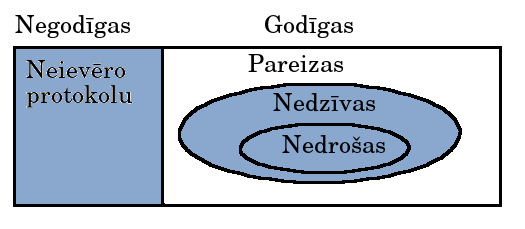
\includegraphics[scale=0.5]{teorija/node-fail.jpg}
    \caption{Venna diagramma virsotņu stāvokļiem}
\label{fig:node-fail}
\end{figure}

Par FBA $\bra{V}{Q}$ sauc virsotņu kopu $V$, kur katrai virsotnei $v\in V$ ir definētas kopas ar virsotnēm $Q(v)$, kas spēj pārliecināt $v$ par vienbalsību. Par \textbf{kvorumu} sauc kopu ar virsotnēm $U$, kurai izpildās īpašība
\begin{equation*}
    \forall v \in U \;\exists q \in Q(v) \;:\; q \subset U
\end{equation*}
Parastā Bizantijas vienošanās ir speciālgadījums, kad $\forall v_1,v_2\in V \;:\; Q(v_1) = Q(v_2)$, un nav jēgpilni runāt par nedzīvām vai nedrošām virsotnēm.
Ja $\bra{V}{Q}$ visu kvorumu šķēlums ir netukšs, tad saka, ka tai ir \textbf{vienots kvorums}. Pieņemsim, ka $V'\subset V$ ir visu godīgo virsotņu kopa un $Q'(v) = \left\{ x\cap V' | x\in Q(v) \right\}$, ja FBA $\bra{V'}{Q'}$ ir vienots kvorums, tad $\bra{V}{Q}$ spēs pieņemt vienotu lēmumu.\cite{mazieres15}

Atšķirībā no iepriekšējām vienprātības metodēm šeit virsotnēm nav nekādās iniciatīvas uzturēt sistēmu.
Stellar veidotāji paredz, ka būs pietiekami daudz sabiedriskā darba darītāju, jo tas nav pārāk dārgi, bet Ripple paredz, ka sistēmu uzturēs tās pašas bankas, kuras to izmantos.

\subsubsection{Proof-of-work alternatīvas}
Galvenokārt alternatīvas tiek meklētas, jo \textit{proof-of-work} uzturēšana prasa daudz elekrtoenerģijas, bet izmantojot vienprātības algoritmus, kuri nebalstās uz sarežģītu problēmu risināšanu, ķēde tiek pakļauta uz vēstures balstītiem uzbrukumiem. Viena no alternatīvām ir izmantot uzdevumus, kuru risināšana aizņem daudz vietas atmiņā, bet nav tik skaitliski ietilpīga.\cite{dziembowski15} Tādējādi tiek risināta ne tikai elekrtoenerģijas patēriņa problēma, bet arī centralizācijas problēma, jo ar specializētām iekārtām nevar iegūt vērā ņemamu priekšrocību. Šādi algoritmi pazīstami ar nosaukumu \textit{proof-of-space} vai \textit{proof-of-storage}.

Vēl citas savdabīgas metodes balstās uz interneta joslas platumu kā ierobežotu resursu. Viena no tām ir \textit{proof-of-DDoS}, kurā virsotnes pēc cita algoritma vienojas, kuram tīmekļa serverim uzbrukt, un tad veic uz šo serveri atkārtotus savienojuma pieprasījumus, līdz ir iegūts savienojuma apstiprinājums ar vēlamām īpašībām, piemēram, hash vērtība ir mazāka par noteiktu vērtību. Šī metode balstās uz citām centralizācijas problēmām kā TLS sertifikātu autoritātēm domēnu validēšanai, un tiek izdarīts pieņēmums, ka DDoS uzbrukuma upuris nesadarbojas ar kādu konkrētu virsotni.\cite{wustrow16}

